
% NOTES (DONE):
%   - Use figures to explain the RCC and Intermediate prioritization algorithms. Its not clear now; too much text 
\begin{frame}{Prioritization algorithms \parencite{hartig2016walking}}
  \begin{block}{Non-adaptive}
    \begin{itemize}
        \item Breadth-first (default), depth-first, random prioritization
    \end{itemize}
  \end{block}
  \begin{block}{Graph-based}
        \begin{itemize}
        \item In-degree, PageRank score
    \end{itemize}
  \end{block}
\end{frame}

\begin{frame}{Prioritization algorithms: Result Contribution-Based (RCC)}
    \begin{columns}[T] % T aligns columns at the top
        % Left column: Image
        \begin{column}{0.6\textwidth} % Adjust width as needed
            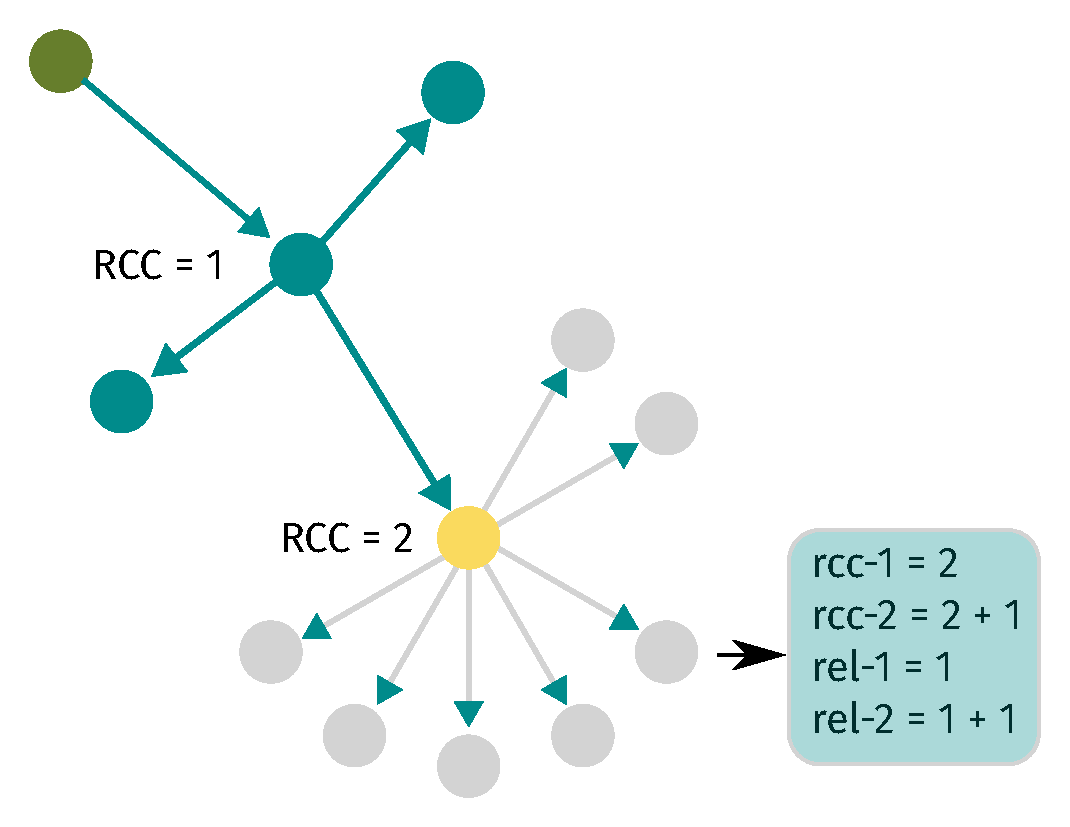
\includegraphics[width=\linewidth]{images/rcc-based.pdf} % replace with your image file
        \end{column}

        % Right column: Text
        \begin{column}{0.4\textwidth} % Adjust width as needed
            \begin{itemize}
                \item Nodes adaptively scored according to the number of results they contribute to
                \item Called \emph{rcc-1}, \emph{rcc-2}, \emph{rel-1}, \emph{rel-2}.
            \end{itemize}
        \end{column}
    \end{columns}
\end{frame}

\begin{frame}{Prioritization algorithms: Intermediate Results-based}
    \begin{columns}[T] % T aligns columns at the top
        % Left column: Image
        \begin{column}{0.6\textwidth} % Adjust width as needed
            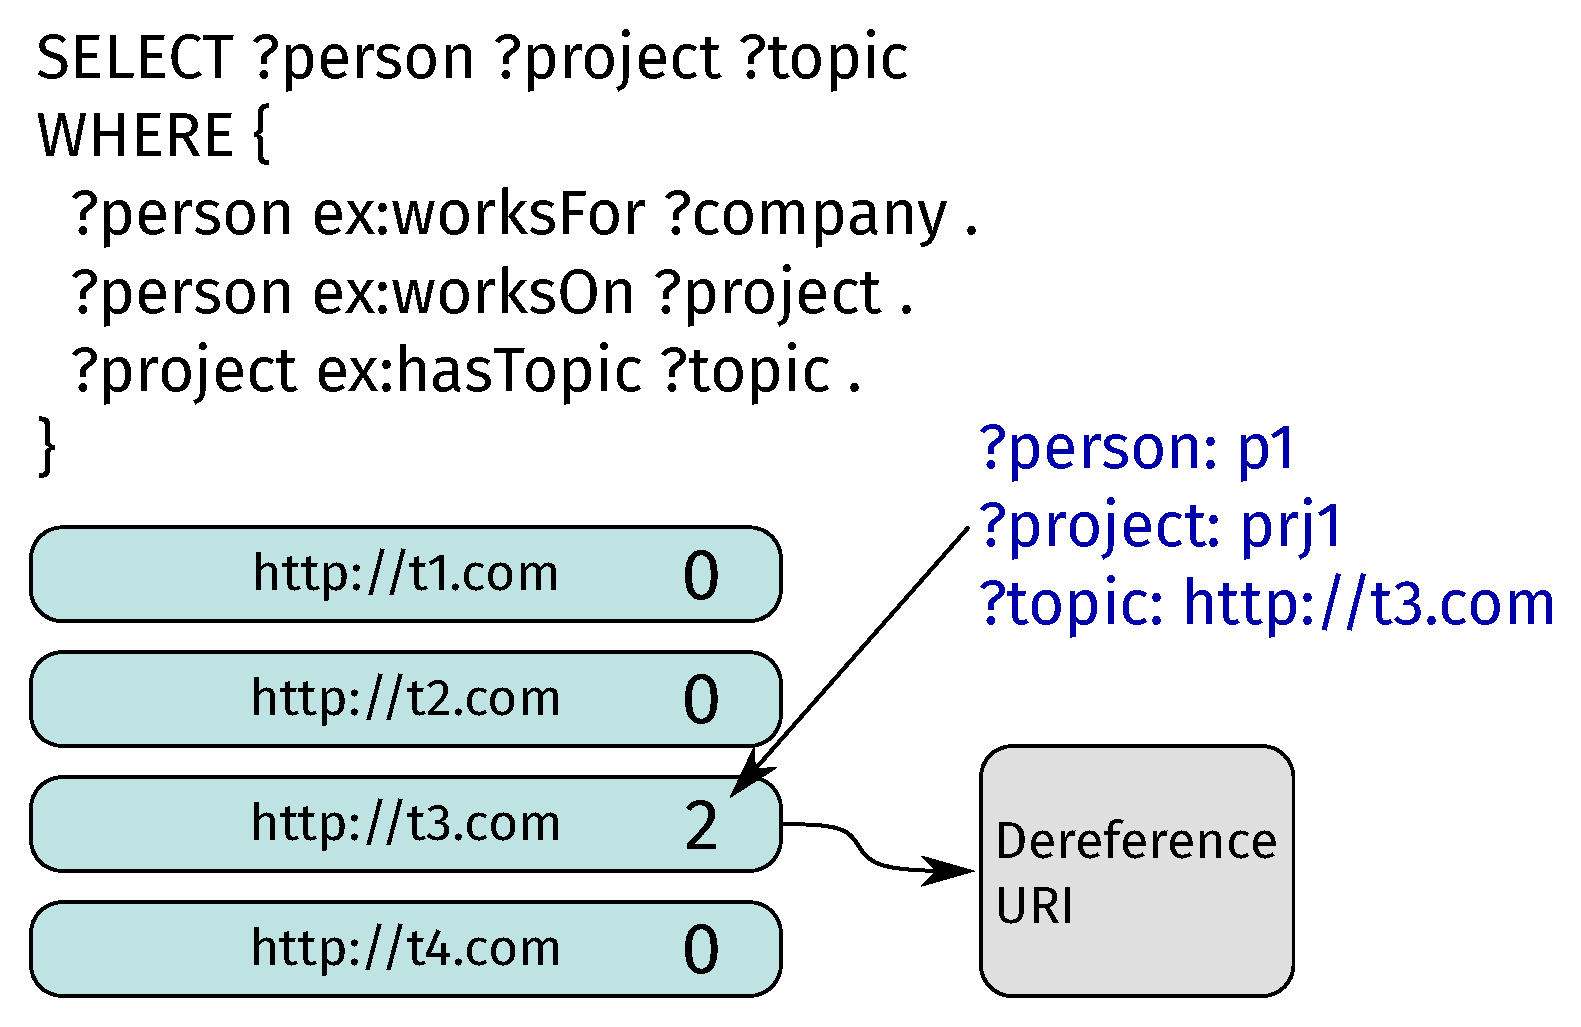
\includegraphics[width=\linewidth]{images/intermediate-results-prioritization.pdf} % replace with your image file
        \end{column}

        % Right column: Text
        \begin{column}{0.4\textwidth} % Adjust width as needed
            \begin{itemize}
                \item Nodes adaptively scored according to their contribution to intermediate results
                \item \emph{IS} with initial priorities of 0, while \emph{ISdcr} sets priority to the priority of the parent node - 1
            \end{itemize}
        \end{column}
    \end{columns}
\end{frame}





\begin{frame}{Prioritization algorithms}
  \begin{block}{Hybrid}
        \begin{itemize}
        \item Multiply intermediate result and RCC-based scoring functions
        \item \emph{is-rcc1}, \emph{is-rcc2}, \emph{is-rel1}, \emph{is-rel2} 
    \end{itemize}
  \end{block}
  \begin{block}{TypeIndex}
        \begin{itemize}
        \item The typeIndexe point to location for resource of specific type
        \item Prioritize TypeIndex first
    \end{itemize}
  \end{block}
  \begin{block}{Oracle}
        \begin{itemize}
        \item Compute RCC in hindsight
        \item Scores are propagated through the shortest path
        \item Serves as optimal performance oracle
    \end{itemize}
  \end{block}

\end{frame}
